\documentclass{article}
\usepackage[utf8]{inputenc}
\usepackage[T1]{fontenc}
\usepackage{graphicx}
\usepackage{amsmath}
\usepackage{wrapfig}
\usepackage[top=1in, bottom=1.25in, left=1.1in, right=1.1in]{geometry}

\title{Reporte - Evaluación 1}
\author{García Monge Itzel Alexia}
\date{08 de Marzo, 2018}

\begin{document}
\maketitle
\section{Descarga de Datos}
Se descargan los archivos que se proporcionan en la página de $PbWorks$, creando una carpeta llamada $Evaluacion1$ dentro de $FisicaComputacionalI$ para guardar los archivos.

Verificamos con $Emcas$ que los archivos descargados se encuentran en buen estado. Ya que los datos no necesitan de un reacomodo o filtro, la limpieza de datos puede llevarse acabo con $Jupyter Notebook$, así que procedemos a abrir una terminal en la carpeta recién creada y abriendo el kernel.

\section{Jupyter Notebook}
\subsection{Limpieza de datos}
Se abre un nuevo Notebook de Python3 y se descargan las bibliotecas necesarias, como \textbf{numpy}, \textbf{pandas}, \textbf{matplotlib}, y \textbf{datetime}. Leemos los archivos descargados, llamando al archivo sargento como $dfsar$, mientras que el archivo sargento-salinidad fue llamado $dfsal$. Los archivos deben empezar y terminar con la misma fecha y hora, así que los leemos con pandas, llamando al archivo sargento como $dfsar$ y le ordenamos que se salte las primeras tres líneas de su documento, mientras que el archivo sargento-salinidad fue llamado $dfsal$ y se le ordenó saltar las primeras dos líneas. Con esto, ambos archivos comienzan en la misma fecha y hora.

Al saltar las líneas iniciales estamos borrando los títulos de las columnas, por lo que necesitamos reincorporarlas con:

\begin{verbatim}
dfsal.columns=['#','Date Time GMT 7','Cond High Rng S/cm','TempC','Specific Conductance 
S/cm','Salinity']
dfsar.columns=['#','Date Time GMT 7','Abs Pres kPa','TempC','WaterLevel']
\end{verbatim}

Como los dos archivos, aunque tengan algunos datos similares, no comparten todos los datos es importante tener cuidado con el nombre que se le otorga a cada columna. 

Ahora falta que ambos archivos acaben en la misma fecha y hora, observando que solamente difieren por una hora de más encontrada en el archivo de $dfsar$, borránodse con:

\begin{verbatim}
dfsar=dfsar[:-1]
\end{verbatim}

Así, ambos documentos están completamente en sincronía de fecha, obteniendo unas tablas de la forma:

	\begin{center}
    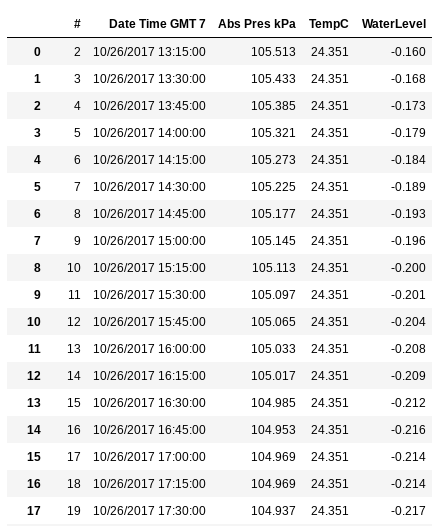
\includegraphics[height=5cm]{headsar.png}{dfsar}
    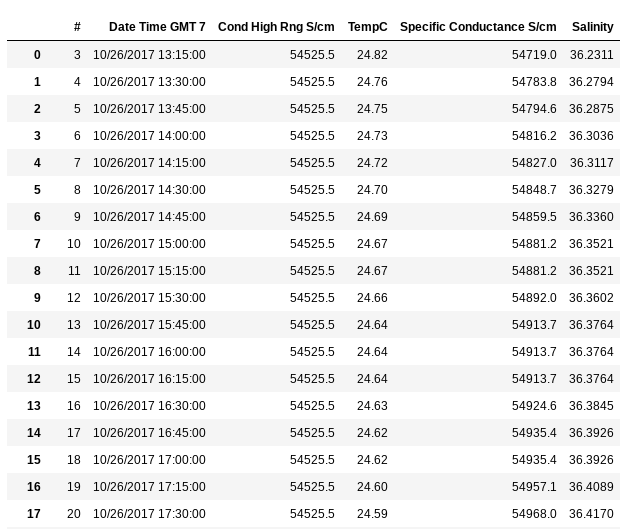
\includegraphics[height=5cm]{headsal.png}{dfsal}
    \end{center}

Pero esto no significa que puedan leerse luego para graficar. Escribimos un $.dtypes$ para observar qué tipo de variables tenemos, encontrando que todas se leen como punto flotante a excepción de la columna $Date$, la cual se lee como objeto en ambos archivos. 

Para cambiar de objeto a punto flotante, usamos el código:

\begin{verbatim}
dfsal['Date'] = pd.to_datetime(dfsal['Date Time GMT 7'], format='%m/%d/%Y %H:%M:%S')
dfsal['month'] = dfsal['Date'].dt.month
\end{verbatim}

En donde $Date$ es la nueva variable que creamos para que se lea como punto flotante de la variable que seleccionamos, en este caso $dfsal$ y dentro de los corchetes seleccionamos la columna que vamos a cambiar a punto flotante, siendo cuidadosos de nombrar el formato como aparece en la columna que nombramos. Con $month$ ahora podemos separar los dos meses y llamarlos por separado a graficar si se deseara.

\section{Gráficas}
\subsection{Boxplot}
Para realizar las gráficas de boxplot es necesario importar la biblioteca \textbf{Seaborn}, lo cual se realiza antes de iniciar. Una vez descargada la biblioteca, se escribe un boxplot que crea dos gráficas, una para octubre y otra para noviembre. 

El primer boxplot se del nivel del mar, así que usamos la variable $dfsar$ para graficar. El segundo boxplot es con respecto a la salinidad, por lo que se usa la variable $dfsal$. La tercera y última gráfica es con la temperatura, ya que ambas variables tienen esta columna podemos usar cualquiera, en este caso se eligió graficar la varibale $dfsar$.

Las gráficas obtenidas son:

	\begin{center}
    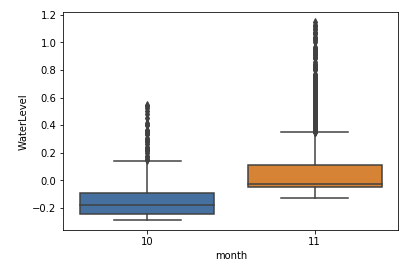
\includegraphics[height=5cm]{boxwat.png}{Nivel del Mar}
    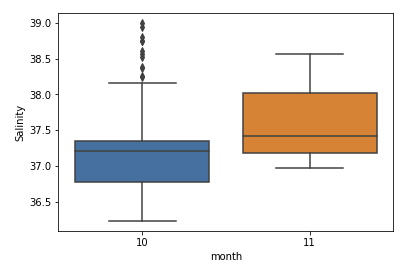
\includegraphics[height=5cm]{boxsalt.png}{Salinidad}
    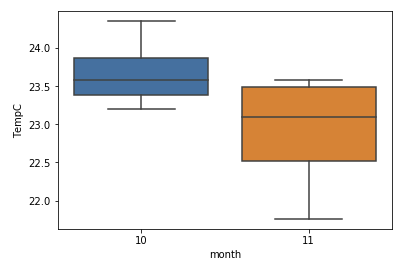
\includegraphics[height=5cm]{boxtemp.png}{Temperatura}
    \end{center}

Si se quiere saber con más detalle el valor de los datos, se usa el comando $.describe()$ para obtener los valores precisos sobre la los cuartiles, la media, el número de datos, entre otros. Los valores de los archivos son:

	\begin{center}
    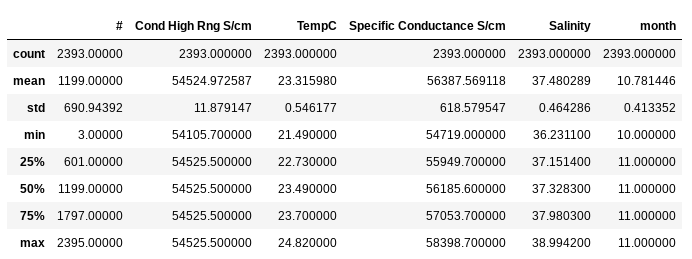
\includegraphics[height=5cm]{resal.png}{Resumen de datos: dfsal}
    \end{center}
	
    \begin{center}
    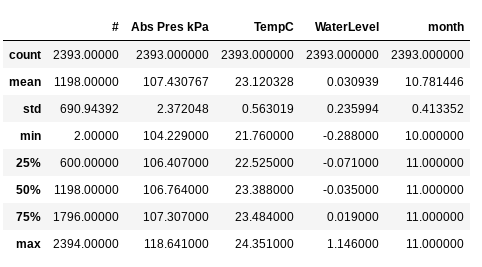
\includegraphics[height=5cm]{resar.png}{Resumen de datos: dfsar}
    \end{center}
    
\subsection{Regresión Lineal}
Para realizar las gráficas de regresión lineal se sigue usando la biblioteca \textbf{Seaborn}. La primera gráfica que se nos pide dice quiere que sea una relación entre el nivel del agua y la salinidad. Para poder graficar esta regresión debemos concatar ambas variables, ya que un valor se encuentra en cada una. Para concatar ambas variables se crea una variable nueva que vaya a guardar la información de ambos.

Para las siguientes dos gráficas de regresión no se necesita concatar ni usar la grafica concatada, pues nos piden una gráfica con ajuste lineal del nivel de mar y temperatura del agua, valores que podemos encontrar en la variable $dfsar$; mientras que la tercera gráfica nos pide una regresión lineal de la salinidad y la temperatura, valores que se encuentran en la variable $dfsal$.

Las gráficas adquieren la forma de:

	\begin{center}
    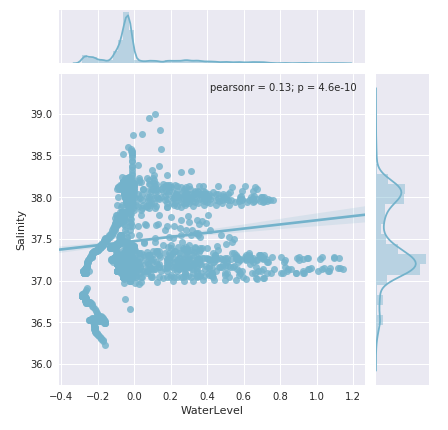
\includegraphics[height=5cm]{regd3.png}{Nivel del Mar}
    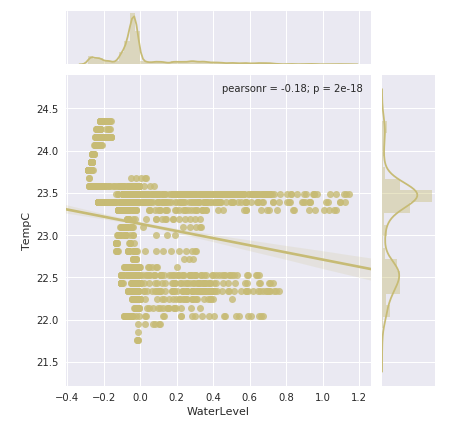
\includegraphics[height=5cm]{regsar.png}{Salinidad}
    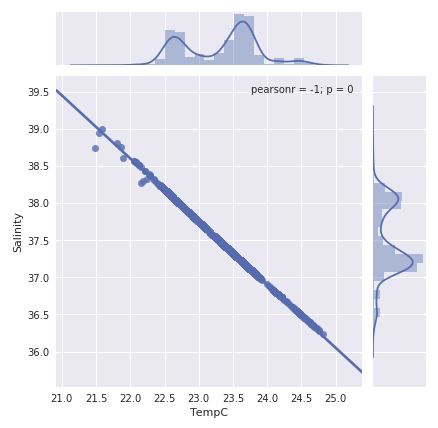
\includegraphics[height=5cm]{regsal.png}{Temperatura}
    \end{center}

\subsection{Gráficas Independientes}
Además de \textbf{Seaborn} todavía tenemos otra biblioteca con la que podemos graficar relaciones. Se quiere graficar la relación que tiene la temperatura, la salinidad y el nivel del agua como función del tiempo de manera independiente. Para eso, solo necesitamos de \textbf{matplotplib}, creando una nueva variable que será la gráfica y obteniendo las relaciones siguientes:

	\begin{center}
    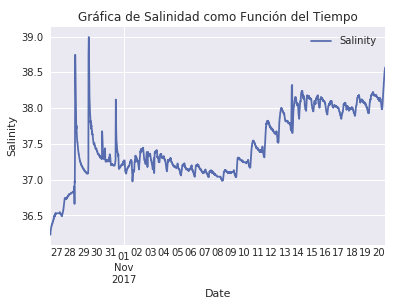
\includegraphics[height=5cm]{lineal1.png}
    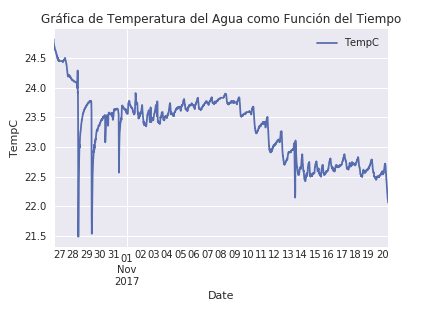
\includegraphics[height=5cm]{lineal2.png}
    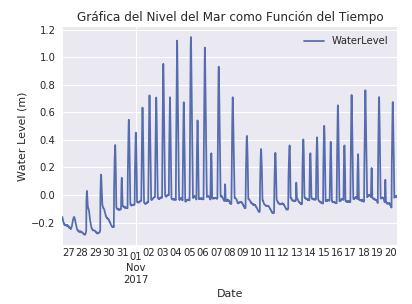
\includegraphics[height=5cm]{lineal3.png}
    \end{center}

\subsection{Doble Eje}
Cuando se desea graficar de forma que no ambos valores se encuentren en el eje $y$, y no de la manera convencional eje $x$ con eje $y$, se debe importar una nueva biblioteca llamada \textbf{pylab}. Con este biblioteca puedes seleccionar qué quieres que vaya en el lado izquierdo del eje $y$ y qué deseas que vaya en el lado derecho, construyendo un código, por ejemplo, de la forma:

\begin{verbatim}
from pylab import figure, show, legend, ylabel
fig1 = figure()

ax1 = fig1.add_subplot(111)
line1 = ax1.plot(dfconjunto['Salinity'], 'b-')
ylabel("Salinity")

ax2 = fig1.add_subplot(111, sharex=ax1, frameon=False)
line2 = ax2.plot(dfconjunto['WaterLevel'], 'xr-')
ax2.yaxis.tick_right()
ax2.yaxis.set_label_position("right")
ylabel("Water Level")

show()
\end{verbatim}

Se realizaron dos gráficas de doble eje, una con nivel del mar y salinidad--la cual requirió usar la variable $dfconjunto$ una vez más--y la segunda con temperatura y nivel del mar.

	\begin{center}
    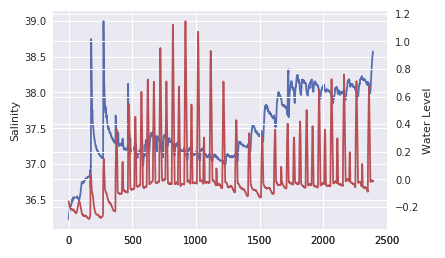
\includegraphics[height=7cm]{dobd3.png}
    \end{center}

	\begin{center}
	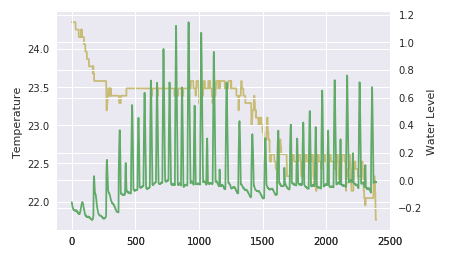
\includegraphics[height=7cm]{dobd2.png}
	\end{center}
    
\subsection{Límites}
A las gráficas recién creadas de doble eje se les quiere tener graficadas de una manera aún más específica, pidiendo que de todos los días de los dos meses que se tienen disponibles, se seleccionen 5. Lo que al principio puede complicar es el hecho de que se pida una restricción que trata con las fechas cuando ninguno de los ejes graficados lo son, pero se resuelve fácilmente al agregar la fecha en el eje $x$ inferior no utilizado, usando tres variables en lugar de dos al escribir el código de la forma:

\begin{verbatim}
fig, ax1 = plt.subplots()
x=dfsal['Date']
Sal=dfconjunto.Salinity
Water=dfconjunto.WaterLevel

ax1.plot(x,Sal,'g-', label='Salinity'); plt.legend(loc='upper left')
ax1.set_xlabel('Date')
ax1.set_ylabel('Salinity (ppt)')

ax2 = ax1.twinx()
ax2.plot(x, Water, 'c-', label='WaterLevel'); plt.legend(loc='upper right')
ax2.set_ylabel('Water Level (m)')

fig.tight_layout()
plt.xlim(("2017-10-26 13:00:00","2017-10-30 13:00:00"))
plt.show()
\end{verbatim}

Y obteniendo unas gráficas más claras.

	\begin{center}
    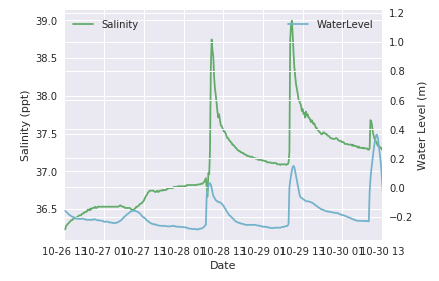
\includegraphics[height=7cm]{ejey1.png}
    \end{center}
	
    \begin{center}
    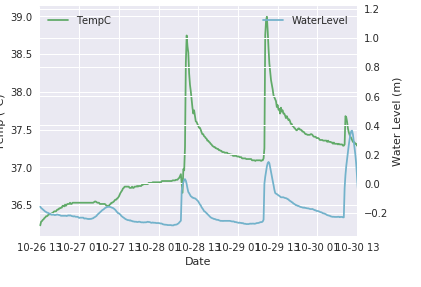
\includegraphics[height=7cm]{ejey2.png}
    \end{center}
	
\end{document}
